
\section{Transforming SeismoCloud to be cloud-ready}

\begin{frame}{First step: Split components and dockerize}
We have three different components with different requirements:

\begin{itemize}
  \item \textbf{SeismoCloud core} (MQTT broker, SeismoCloud controller, database):
  high availability, high elasticity and geo-distributed, \textit{high priority}
  \item \textbf{API}: high availability and scalability
  \item \textbf{Website}: scalability, \textit{low priority}
\end{itemize}

They have been separated and re-written as stateless Docker containers. This is
a strategic decision in order to simplify the cloud deployment and multi-tier.
\end{frame}


\begin{frame}{First step: Split components and dockerize}
\centering
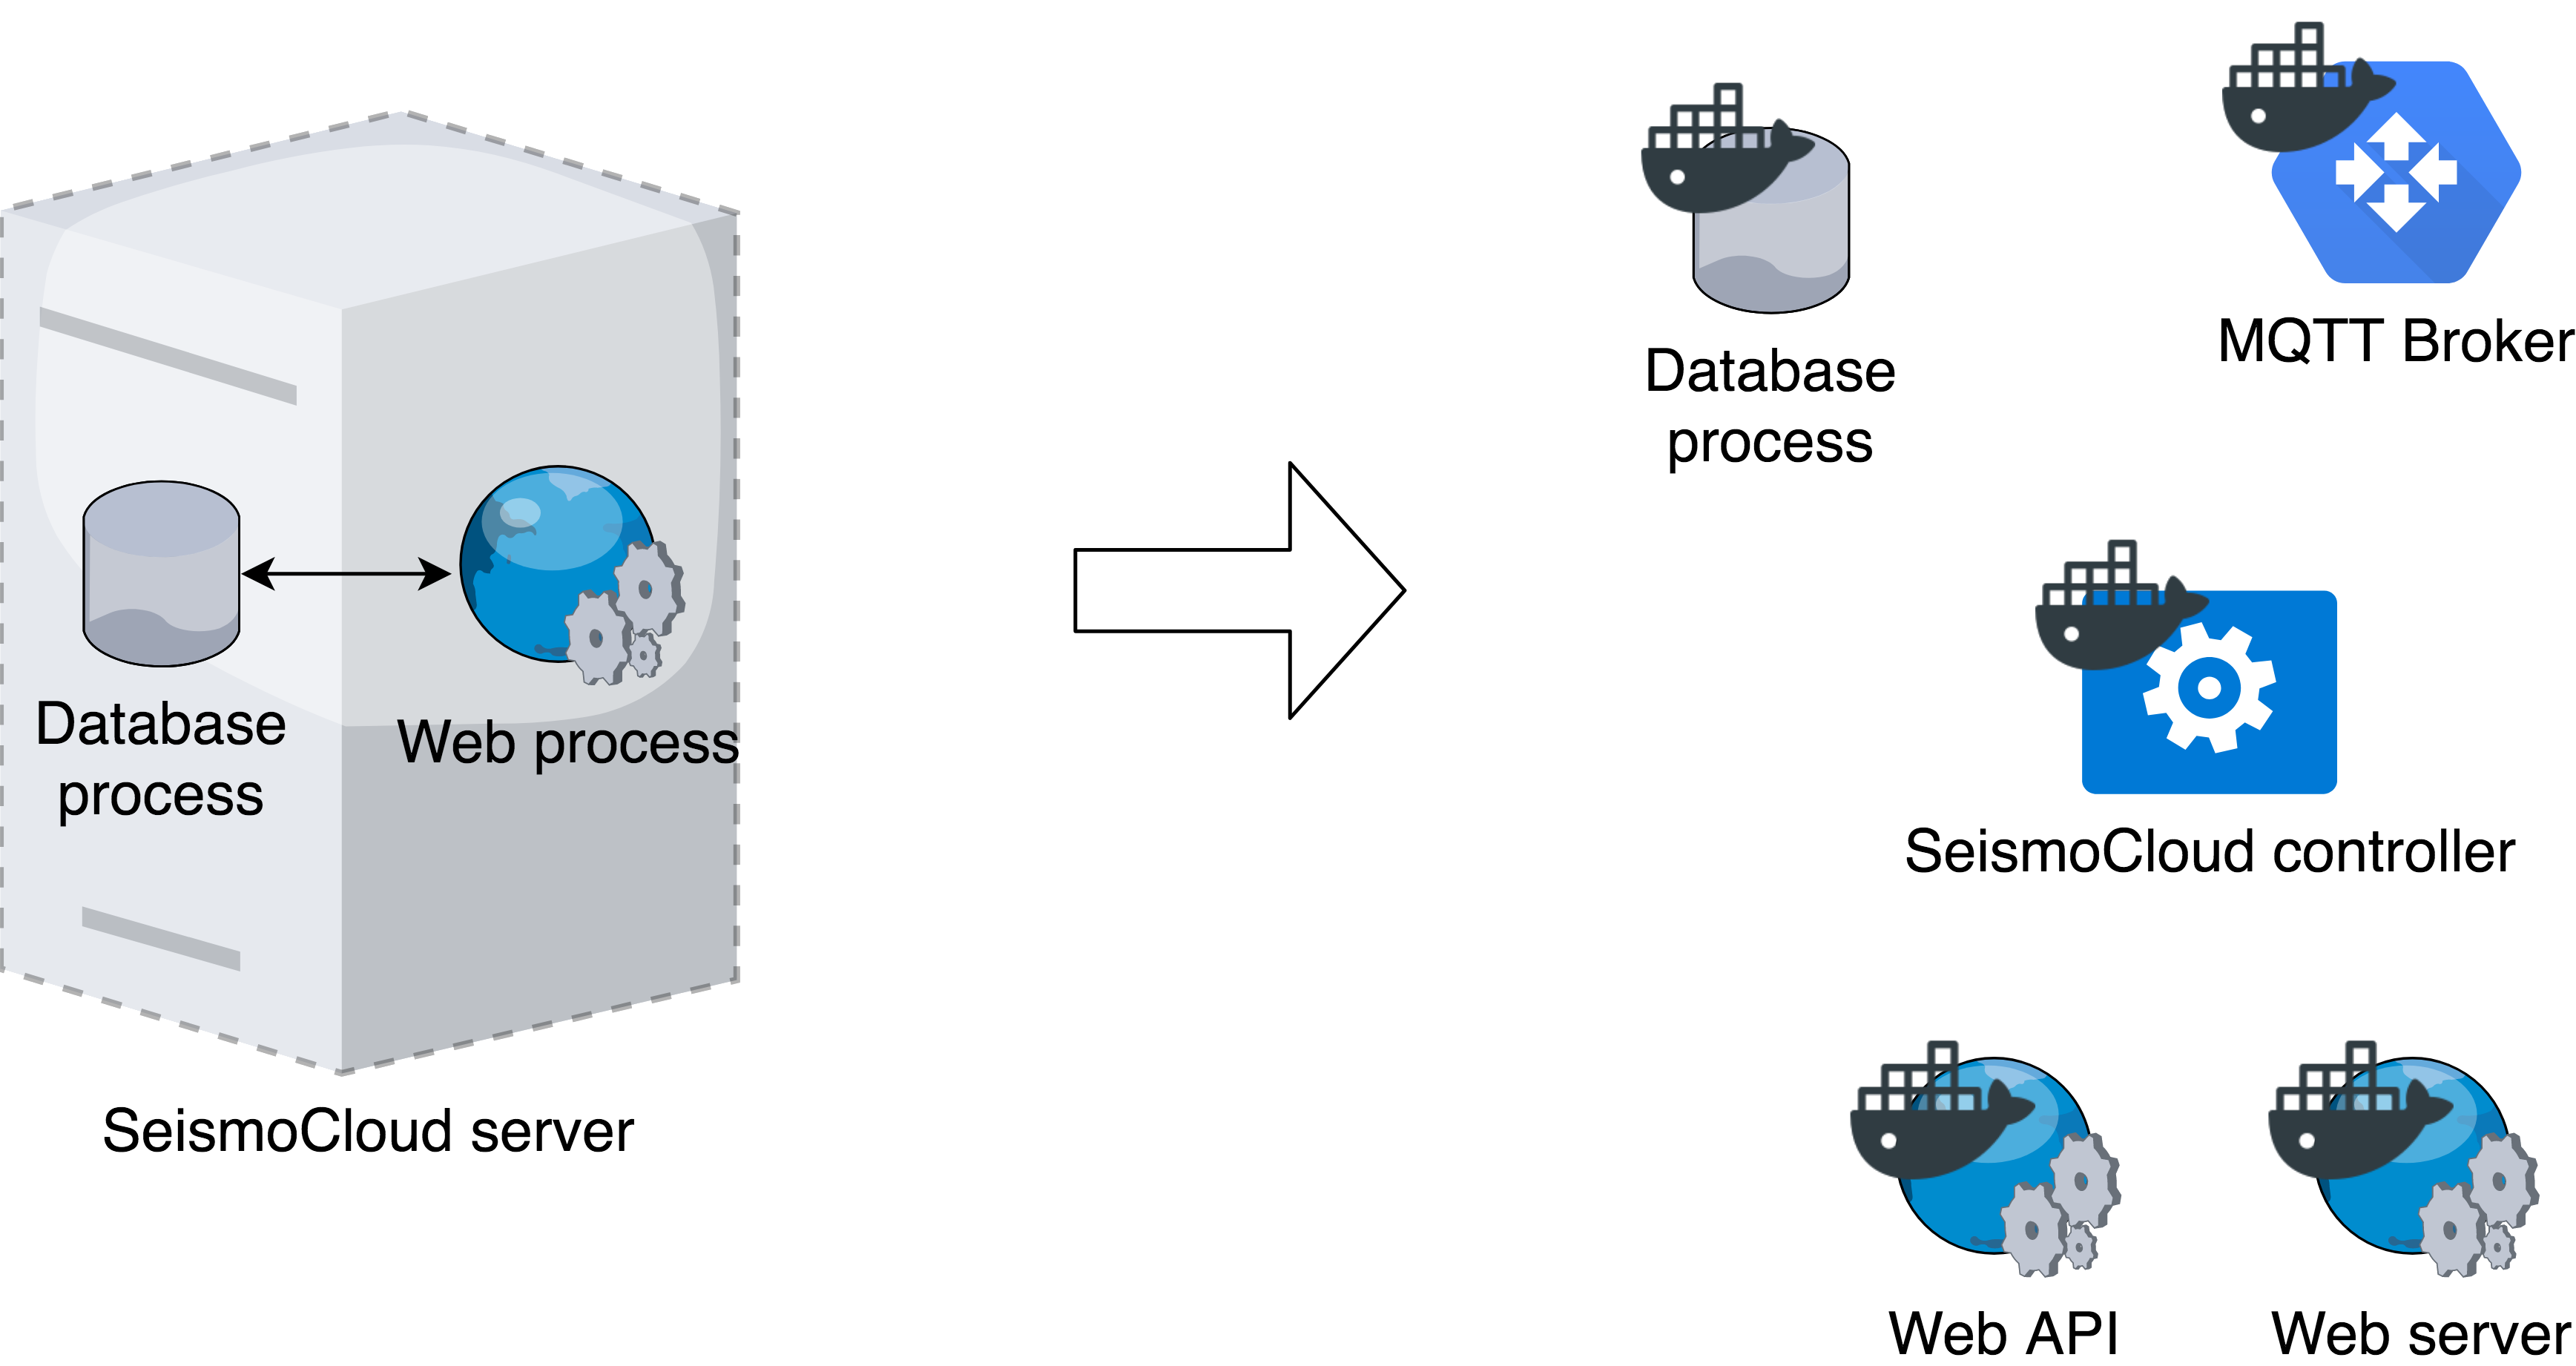
\includegraphics[width=0.9\textwidth]{scs-split-components}
\end{frame}


\begin{frame}{Second step: From MySQL to...}
A \textbf{core} component of SeismoCloud system is the data storage. We store
both technical data (eg. IoT device informations) and sensor data (such as
strongness of seismic wave acceleration).

The current system is based on a Relational DMBS named \textit{MySQL}.

As every R-DBMS, its capability to scale is very limited due to CAP theorem: a
R-DBMS prioritize \textit{Consistency} over \textit{Availability} during a
\textit{Partition}.
\end{frame}


\begin{frame}{CAP theorem}
\centering
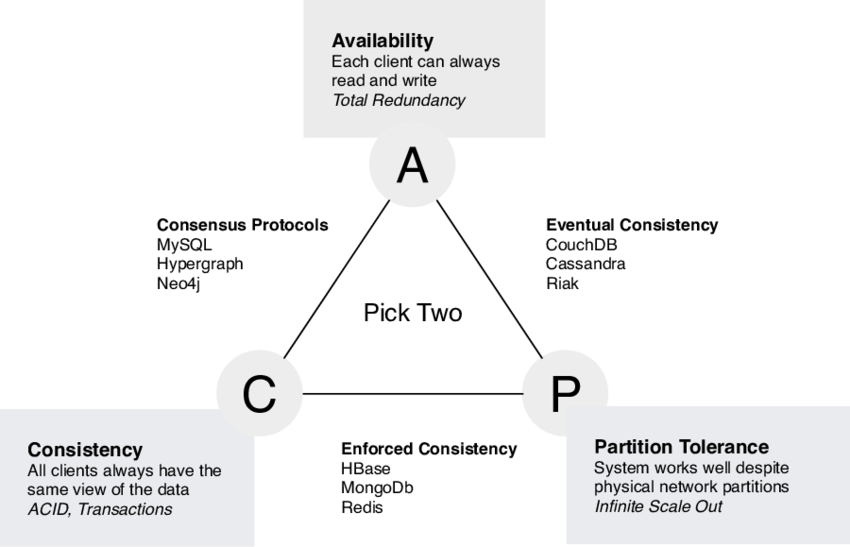
\includegraphics[keepaspectratio=true,width=\textwidth]{CAP-Theorem}
\end{frame}


\begin{frame}{Second step: From MySQL to Apache Cassandra / Redis}
For some storage \textit{actions} we need a highly scalable system that
doesn't need to be consistent at every moment. Examples of these situation are:

\begin{itemize}
  \item Store \textit{historical} data about earthquake waves
  \item Store device performance data
  \item Handle system and device logging
  \item Handle volatile data (such as session databases)
\end{itemize}

This needs are addressed with NoSQL products named \textit{Apache Cassandra} and
\textit{Redis}.
\end{frame}


\begin{frame}{Future SeismoCloud architecture}
\centering
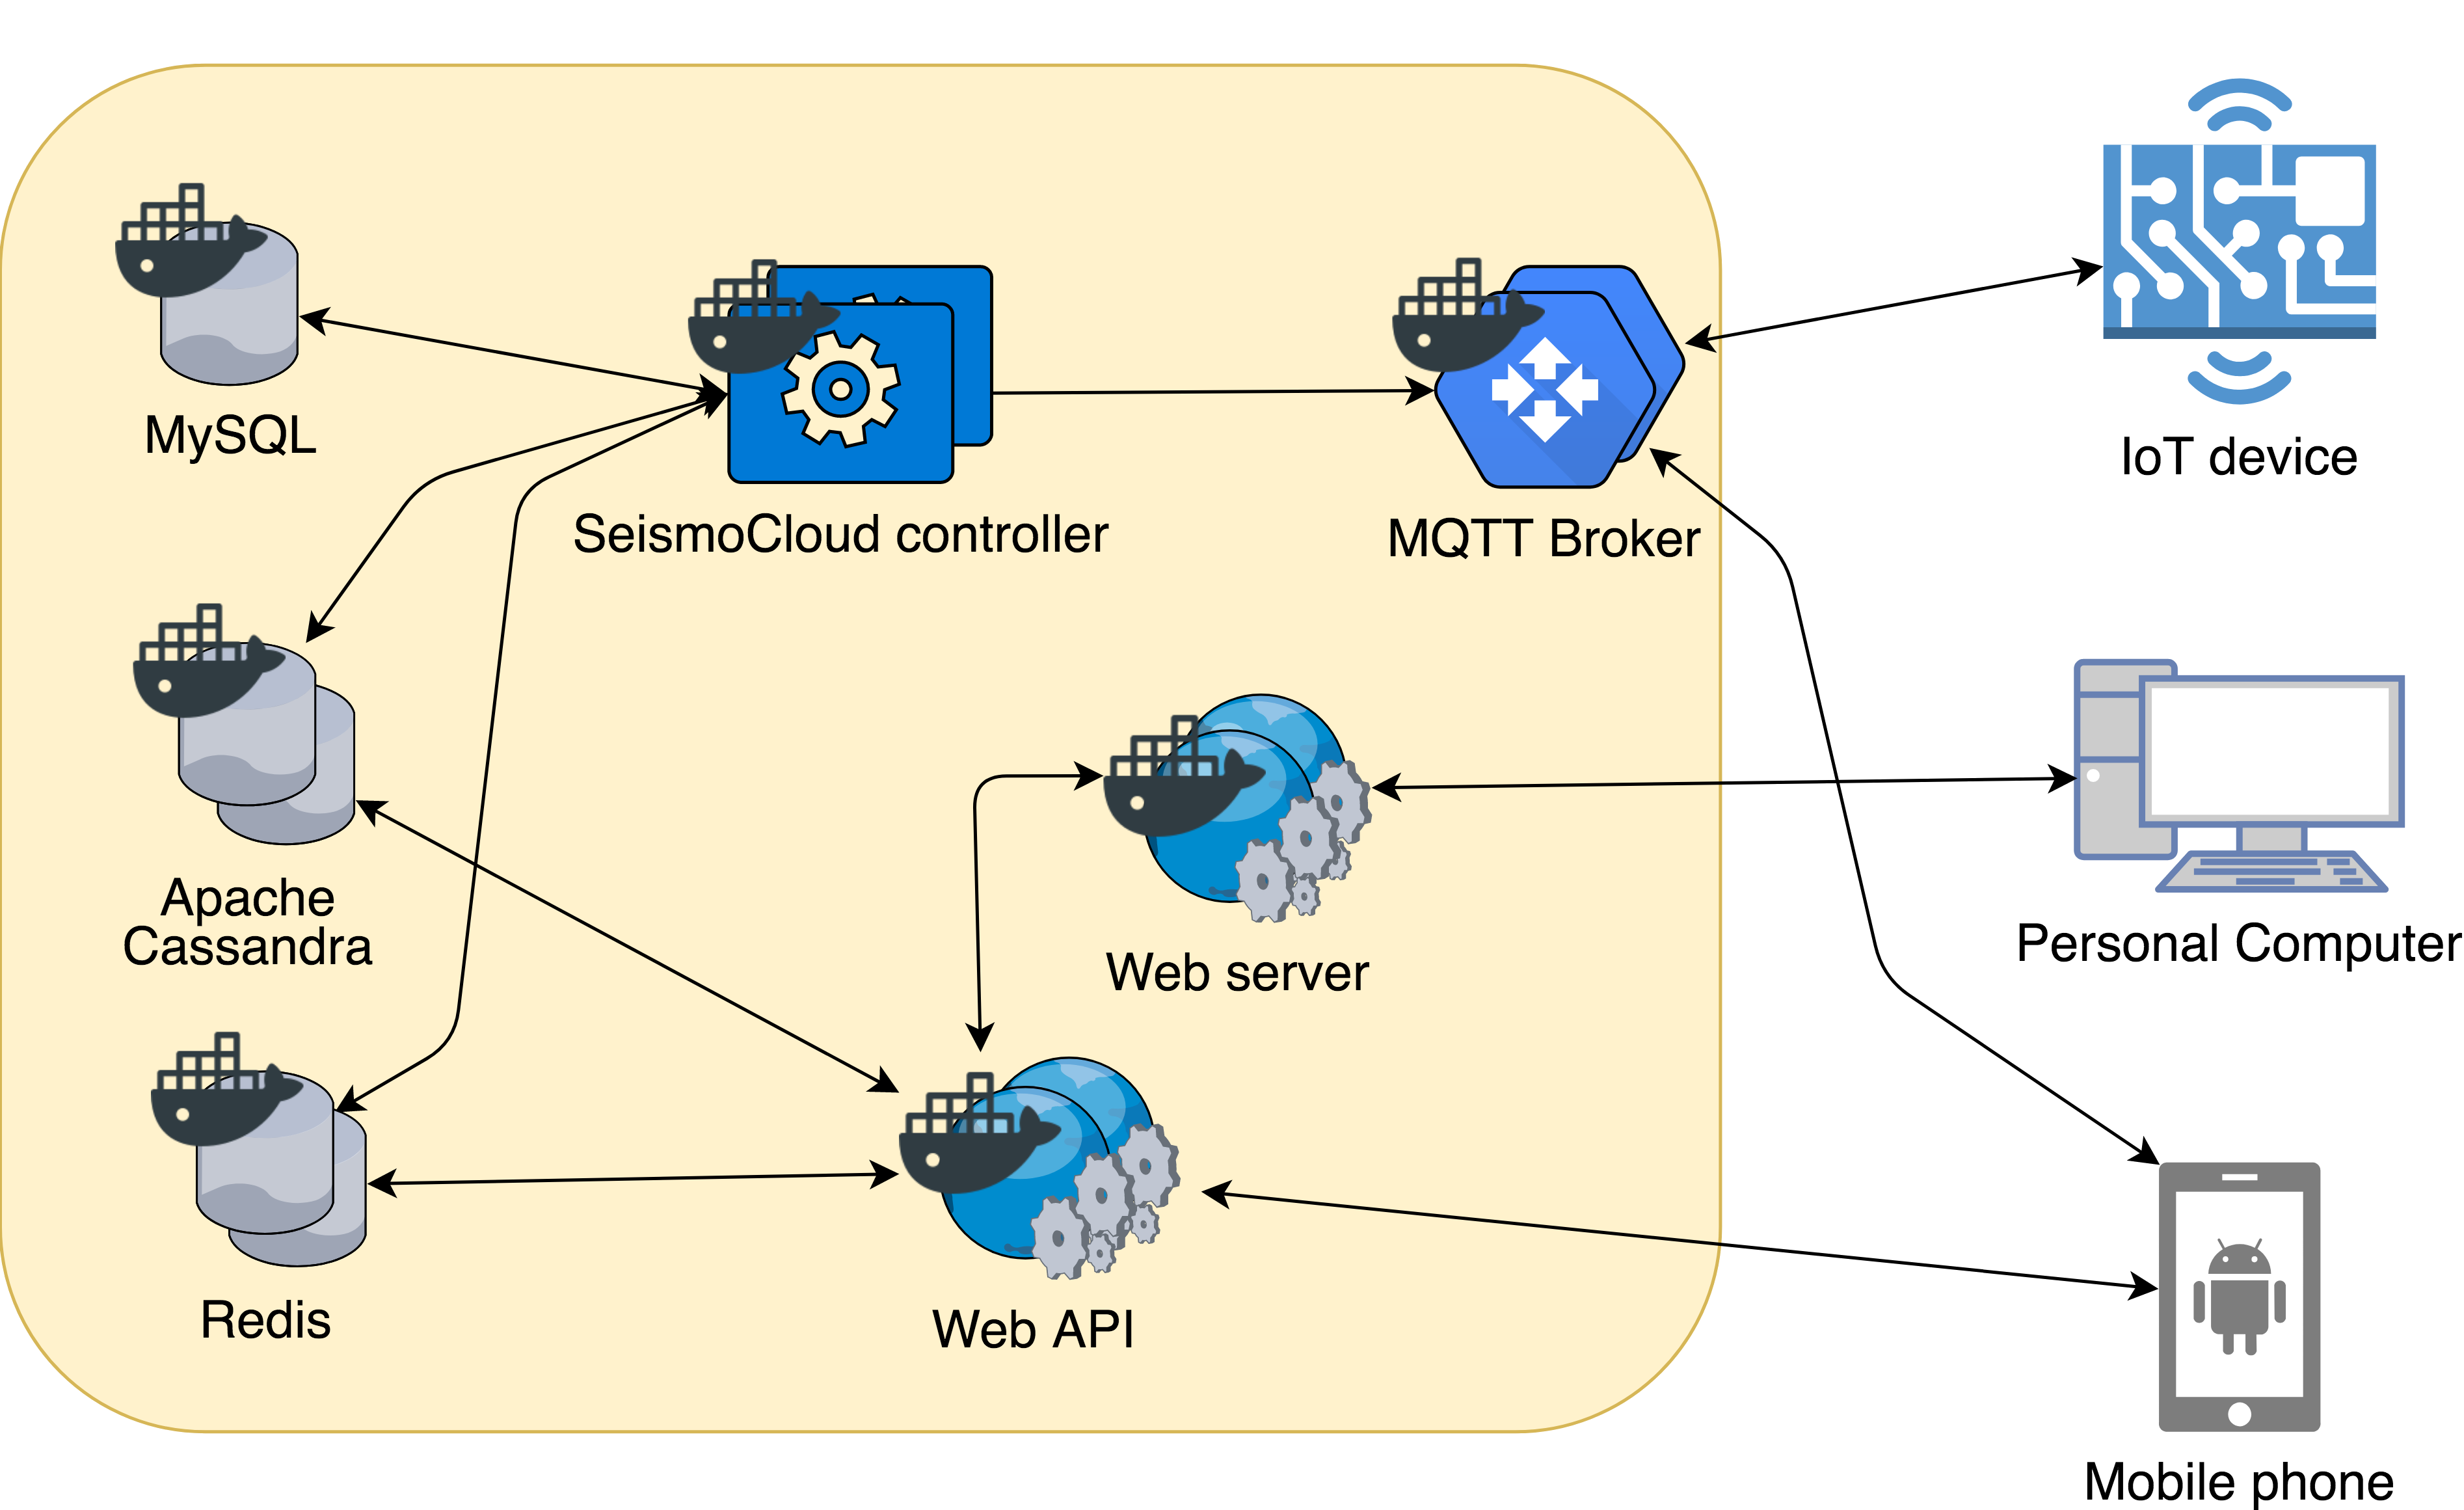
\includegraphics[keepaspectratio=true,width=\textwidth]{scs-future-architecture}
\end{frame}


\begin{frame}{Refactoring costs}

	The overall refactoring took nearly a month of a 1-person development, and will
	require an estimated time of 2 week of testing (before going into production).

	\vspace{3em}

	The total estimated cost for this operation is 7500 € (250 € / workday)

\end{frame}
